\documentclass[11pt,fleqn]{article}
\usepackage[letterpaper]{geometry}
\usepackage{graphicx}    % needed for including graphics e.g. EPS, PS
\usepackage{amsmath}
\usepackage{xfrac}
\usepackage[version=4]{mhchem}
\usepackage{listings}
\usepackage{hyperref}
\usepackage{wrapfig}
\usepackage{empheq}
\usepackage{capt-of}



% To use UTF-8 characters
\usepackage[utf8x]{inputenc}
% \DeclareUnicodeCharacter{207A}{$^+$}
% \DeclareUnicodeCharacter{207B}{$^-$}







% color def PYTHON CODE
\usepackage{color}
\definecolor{darkred}{rgb}{0.6,0.0,0.0}
\definecolor{darkgreen}{rgb}{0,0.50,0}
\definecolor{lightblue}{rgb}{0.0,0.42,0.91}
\definecolor{orange}{rgb}{0.99,0.48,0.13}
\definecolor{grass}{rgb}{0.18,0.80,0.18}
\definecolor{pink}{rgb}{0.97,0.15,0.45}

% listings
\usepackage{listings}

% General Setting of listings
\lstset{
	aboveskip=1em,
	breaklines=true,
	abovecaptionskip=-6pt,
	captionpos=b,
	escapeinside={\%*}{*)},
	frame=single,
	numbers=left,
	numbersep=15pt,
	numberstyle=\tiny,
}
% 0. Basic Color Theme
\lstdefinestyle{colored}{ %
	basicstyle=\ttfamily,
	backgroundcolor=\color{white},
	commentstyle=\color{green}\itshape,
	keywordstyle=\color{blue}\bfseries\itshape,
	stringstyle=\color{red},
}
% 1. General Python Keywords List
\lstdefinelanguage{PythonPlus}[]{Python}{
	morekeywords=[1]{,as,assert,nonlocal,with,yield,self,True,False,None,} % Python builtin
	morekeywords=[2]{,__init__,__add__,__mul__,__div__,__sub__,__call__,__getitem__,__setitem__,__eq__,__ne__,__nonzero__,__rmul__,__radd__,__repr__,__str__,__get__,__truediv__,__pow__,__name__,__future__,__all__,}, % magic methods
	morekeywords=[3]{,object,type,isinstance,copy,deepcopy,zip,enumerate,reversed,list,set,len,dict,tuple,range,xrange,append,execfile,real,imag,reduce,str,repr,}, % common functions
	morekeywords=[4]{,Exception,NameError,IndexError,SyntaxError,TypeError,ValueError,OverflowError,ZeroDivisionError,}, % errors
	morekeywords=[5]{,ode,fsolve,sqrt,exp,sin,cos,arctan,arctan2,arccos,pi, array,norm,solve,dot,arange,isscalar,max,sum,flatten,shape,reshape,find,any,all,abs,plot,linspace,legend,quad,polyval,polyfit,hstack,concatenate,vstack,column_stack,empty,zeros,ones,rand,vander,grid,pcolor,eig,eigs,eigvals,svd,qr,tan,det,logspace,roll,min,mean,cumsum,cumprod,diff,vectorize,lstsq,cla,eye,xlabel,ylabel,squeeze,}, % numpy / math
}
% 2. New Language based on Python
\lstdefinelanguage{PyBrIM}[]{PythonPlus}{
	emph={d,E,a,Fc28,Fy,Fu,D,des,supplier,Material,Rectangle,PyElmt},
}
% 3. Extended theme
\lstdefinestyle{colorEX}{
	basicstyle=\ttfamily,
	backgroundcolor=\color{white},
	commentstyle=\color{darkgreen}\slshape,
	keywordstyle=\color{blue}\bfseries\itshape,
	keywordstyle=[2]\color{blue}\bfseries,
	keywordstyle=[3]\color{grass},
	keywordstyle=[4]\color{red},
	keywordstyle=[5]\color{orange},
	stringstyle=\color{darkred},
	emphstyle=\color{pink}\underbar,
}









\usepackage{tikz}
\usepackage{tikzpagenodes}
\usetikzlibrary{positioning}

\topmargin -1.5cm        % read Lamport p.163
\oddsidemargin -0.04cm   % read Lamport p.163
\evensidemargin -0.04cm  % same as oddsidemargin but for left-hand pages
%\textwidth 16.59cm
\textwidth 11cm
\textheight 21.94cm 
%\pagestyle{empty}       % Uncomment if don't want page numbers
\parskip 7.2pt           % sets spacing between paragraphs
%\renewcommand{\baselinestretch}{1.5} 	% Uncomment for 1.5 spacing between lines
\parindent 0pt		  % sets leading space for paragraphs


\newcounter{qNum}
\newcommand{\qn}{\refstepcounter{qNum} \theqNum}
\newcounter{qNumH}
\newcommand{\qnH}{\refstepcounter{qNumH}  \textit{Honors} \theqNumH}
\newcommand{\eqn}{\text{\qn) \ }}
\def \dt {\ensuremath{\,\mathrm{d}t}}

\newcommand{\aspace}{ \hspace{1em}\\ \vspace{8em}}

\newcommand{\dx}{\; dx}

\newcommand{\D}[1]{\; d{#1}}

\newcommand{\graphGrid}{
	
\begin{tikzpicture}
	\draw[step=.5cm,gray,help lines] (-5,-5) grid (5,5);
	\draw[step=2.5cm,black,very thin] (-5,-5) grid (5,5);
	\end{tikzpicture}
}

\newcommand{\graphGridAxes}{
	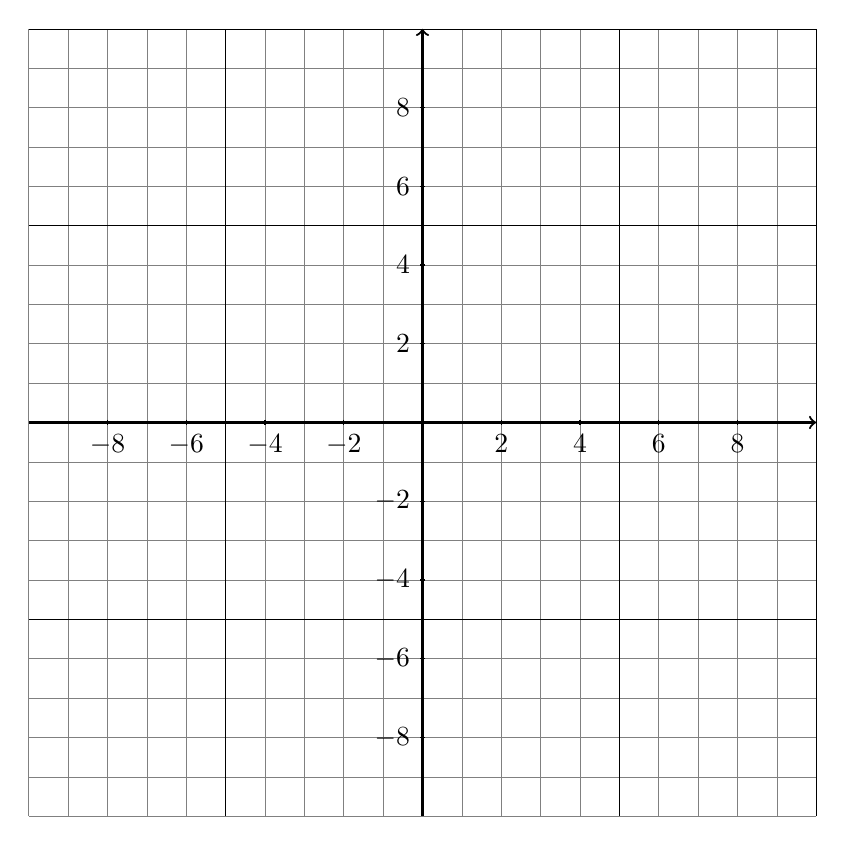
\begin{tikzpicture}
	\draw[step=.5cm,gray,help lines] (-5,-5) grid (5,5);
	\draw[step=2.5cm,black,very thin] (-5,-5) grid (5,5);
	\draw[thick,->] (-5,0) -- (5,0) ;
	\draw[thick,->] (0,-5) -- (0,5) ; 
	\foreach \x in {-8, -6, -4, -2,  2,4, 6, 8}
	\draw (\x*0.5 cm,1pt) -- (\x*0.5 cm,-1pt) node[anchor=north] {$\x$};
	\foreach \y in {-8, -6, -4, -2,  2,4, 6, 8}
	\draw (1pt,\y*0.5 cm) -- (-1pt,\y*0.5 cm) node[anchor=east] {$\y$};
	\end{tikzpicture}
}

\newcommand{\graphGridAxesS}[1]{
	\begin{tikzpicture}
		\draw[step=.5cm,gray,help lines] (-0.5*#1,-0.5*#1) grid (0.5*#1, 0.5*#1);
		\draw[step=2.5cm,black,very thin] (-0.5*#1,-0.5*#1) grid (0.5*#1, 0.5*#1);
		\draw[thick,->] (-#1/2,0) -- (#1/2,0) ;
		\draw[thick,->] (0,-#1/2) -- (0,#1/2) ; 
		\foreach \x in {-8, -6, -4, -2,  2,4, 6, 8}
		\draw (\x*0.5 cm,1pt) -- (\x*0.5 cm,-1pt) node[anchor=north] {$\x$};
		\foreach \y in {-8, -6, -4, -2,  2,4, 6, 8}
		\draw (1pt,\y*0.5 cm) -- (-1pt,\y*0.5 cm) node[anchor=east] {$\y$};
	\end{tikzpicture}
}



%headers
\usepackage{datetime}
\usepackage{fancyhdr}
\pagestyle{fancy}
\lhead{ Name: }
\rhead{\footnotesize Finite Difference Method: Cylindrical Tube (\monthname, \the\year)}
\title{Introduction to the Finite Difference Method: \\ Filling and Draining a Cylindrical Tube}
\author{Lensyl Urbano}



 \begin{document}         
 % Start your text
 
\maketitle



Consider filling a cylinder with water. 


	\begin{tikzpicture}[remember picture,overlay,shift={(current page.east)}]
		\node[anchor=north east,xshift=-2cm](myImage){
			%\centering
			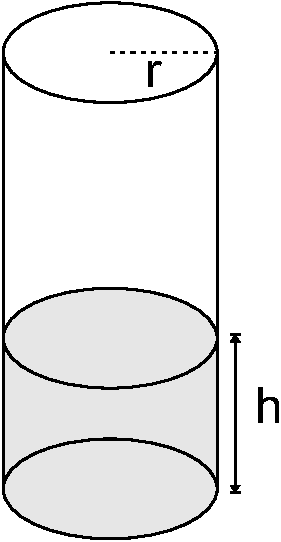
\includegraphics[height=5cm]{cylinder-rh.pdf} 
		};
		\node[inner sep=0pt,text width=0.5\linewidth] (myCaption) [below=of myImage]
	{\captionof{figure}{Cylinder with dimensions. $r$ is the radius and $h$ is the height of water in the tube.}};
	\end{tikzpicture}




The water flows in at a constant rate of 5 cm$^3$/s. The inflow rate ($Q$) can be written as the change in volume ($V$) over the change in time ($t$) (the $\Delta$ symbol represents change):

\textbf{Inflow Rate}
\begin{equation}
	Q = \frac{\Delta V}{\Delta t} = 5 \; cm^3/s
\end{equation}



\section{Filling the Tube Calculations and Equations}

\subsection{Conceptual Physics Approach}

		      
	So, at this inflow rate, after 10 seconds there will be 50 cm$^3$ added to the cylinder.
		\begin{align*}
			 V &= 5 \; cm^3/s \cdot 10 \; s \\
					&= 50 \; cm^3
		\end{align*}
	
	In terms of the equation, the change in volume is equal to the inflow rate ($Q$) times the time period ($ t$).
	  \begin{equation}
	  	\label{Vrate}
	  	 V = Q \cdot t \\
	  \end{equation}
	
	How high will the water have risen in the cylinder in those 10 seconds when 50 cm$^3$ of water was added? Well, we know that the volume of a cylinder is given by the equation:
		\begin{equation}
			V = \pi r^2 h
		\end{equation}
	
	So, if we know the volume and the radius of the cylinder ($r$) we can solve this equation for the height ($h$):
	
	Divide both sides by $\pi r^2$:
		\begin{equation}
			\frac{V}{\pi r^2} = \frac{\pi r^2 h}{\pi r^2}
		\end{equation}
	
	To get:
		\begin{equation}
			\frac{V}{\pi r^2} = h 
		\end{equation}
	
	Which can be rewritten as:
		\begin{equation}
			h = \frac{V}{\pi r^2}  
		\end{equation}
	
	or:
		\begin{equation}
			h = \frac{1}{\pi r^2} V
		\end{equation}
	
	Thus, for our given problem where the radius is 2.25 cm, and the volume of water added is 50 cm$^3$:
		\begin{equation}
			h = \frac{1}{\pi \cdot 2.25^2} \cdot 50 = 3.1 \; \text{cm}
		\end{equation}
	
	
	Now we can substitute for volume using Equation \ref{Vrate} to get:
		\begin{equation}
			h = \frac{1}{\pi r^2} \; Q \cdot t
		\end{equation}
	
	Now, lets rewrite this equation so we just consider what happens over a small time period (call it a \textit{time step} denoted by $\Delta t$). It's the change from moment to moment and results in a small change in height ($\Delta h$). So our final equation becomes:
		\begin{equation}
			\Delta h = \frac{1}{\pi r^2} \; Q \cdot \Delta t
		\end{equation}
	
	Which we rearrange a little to get:
		\begin{empheq}[box=\fbox]{equation}
			\label{dh_eqn}
			\Delta h = \frac{\Delta t}{\pi r^2} \; Q 
		\end{empheq}
	
	Having calculated the change in the height of the water in the cylinder in a given time step ($\Delta t$), for each timestep we calculate the new height of water ($h_{new}$) as the old height plus the change:
		\begin{empheq}[box=\fbox]{equation}
			\label{hnew_eqn}
			h_{new} = h_{old} + \Delta h
		\end{empheq}
	
	We can now use these two equation to create a computer model that gives the height of water in the column over time.
	

\subsection{Using Calculus to Find the Discrete Equations} \label{CodeCalc}

	Same problem--filling a cylinder--but using calculus to end up with the same equations in the end.
	
	Start with the equation for the volume of a cylinder:
		\begin{equation}
			V = \pi r^2 h
		\end{equation}
	
	There are two variables that change with time as the cylinder fills, the volume ($V$) and the height ($h$) since the radius ($r$) does not change. So, if we differentiate this equation with respect to time (implicit differentiation), we get:
		\begin{equation}
			\frac{dV}{dt} = \pi r^2 \frac{dh}{dt} 
		\end{equation}
	
	Solving for $\frac{dh}{dt}$ gives the \textbf{height change equation}:
		\begin{equation}
			\label{eqn:heightChange}
			\frac{dh}{dt} = \frac{1 }{\pi r^2 } \frac{dV}{dt}
		\end{equation}

	The expression $\frac{dh}{dt}$ represents the instantaneous change in height with time: the rate at which height changes at any instant. To write a program to solve this equation we'll \textbf{discretize} the expression by using $\frac{\Delta h}{\Delta t}$:
		\begin{equation}
			\frac{\Delta h}{\Delta t} \approx \frac{dh}{dt} 
		\end{equation}
		
	The $\Delta$ means that we're taking the difference between two discrete value of $h$, so:
		\begin{equation}
			\Delta h = h_2 - h_1
		\end{equation}
	
	Since this is the rate of change over time it can be easier to think of the change in height as the difference between the new height and the old height over the short ($\Delta t$) time period.
		\begin{equation}
			\label{eqn:discrete_h}
			\Delta h = h_{new} - h_{old}
		\end{equation}
	
	So now we rewrite our height change equation (Eqn. \ref{eqn:heightChange}) as:
		\begin{equation}
			\frac{\Delta h}{\Delta t} = \frac{1 }{\pi r^2 } \frac{dV}{dt}
		\end{equation}
		
	which we can solve for the change in height ($\Delta h$):
		\begin{equation}
		\Delta h = \frac{\Delta t }{\pi r^2 } \frac{dV}{dt}
		\end{equation}
	
	Since the inflow rate ($Q$) is the change in volume over time, and it remains constant for our model, we can say:
	
	\textbf{Change in Height Equation}
		\begin{empheq}[box=\fbox]{equation}
			\label{eqn:dh_calc}
			\Delta h = \frac{\Delta t }{\pi r^2 } \; Q
		\end{empheq}
	
	Which is the same equation (Eqn. \ref{dh_eqn}) we found when we took the conceptual approach in the previous section.
	
	Now we substitute in the discrete change for $\Delta h$ (Eqn. \ref{eqn:discrete_h}) to get:
		\begin{equation}
			 h_{new} - h_{old} = \frac{\Delta t }{\pi r^2 } \; Q
		\end{equation}
	
	Which we can solve for the new height:
		\begin{equation}
			h_{new} = h_{old} + \frac{\Delta t }{\pi r^2 } \; Q
		\end{equation}
	
	
	Which is the same as:
	
	\textbf{Height Update Equation}
		\begin{empheq}[box=\fbox]{equation}
			\label{eqn:dh_discrete}
			h_{new} = h_{old} + \Delta h 
		\end{empheq}
	
	We can use the \textbf{Change in Height} (Eqn. \ref{eqn:dh_calc}) and \textbf{Height Update} (Eqn. \ref{eqn:discrete_h}) equations to create a computer model of the height of the water in the cylinder as it fills it up.

\newpage
\section{Code}

	The following example code that solves this water-filling problem uses the \href{https://github.com/lurbano/ezGraph}{ezGraph class} \\ (https://github.com/lurbano/ezGraph) which requires matplotlib and numpy. However, the code in the following section avoids the use of most imported modules, but does not graph.
	
	\subsubsection{Code with Graphical Output}
	
		\textit{water-filling-fd.py}
		\begin{tikzpicture}[remember picture,overlay,shift={(current page.east)}]
			\node[anchor=north east,xshift=-1cm](fillingOutput){
				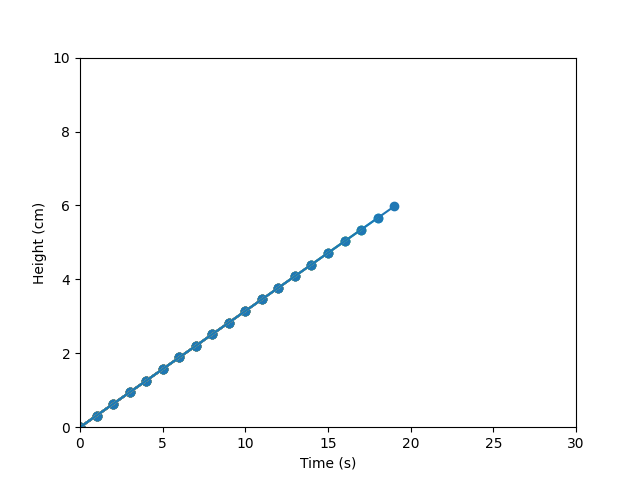
\includegraphics[height=5cm]{water-filling-fd.png} 
			};
			\node[inner sep=0pt,text width=0.5\linewidth] (myCaption) [below=of myImage]
			{\captionof{figure}{\label{fillingModel} Model output: Graph of height of water in the column over time when filling the cylinder.  }};
		\end{tikzpicture}
	
		\lstinputlisting[language=Python, frame=single]{../water-filling-fd.py}

	
	
%	\begin{figure}[h] 
%		\caption{Model output: Graph of height of water in the column over time when filling the cylinder.}
%		\centering
%		\label{fillingModel}
%		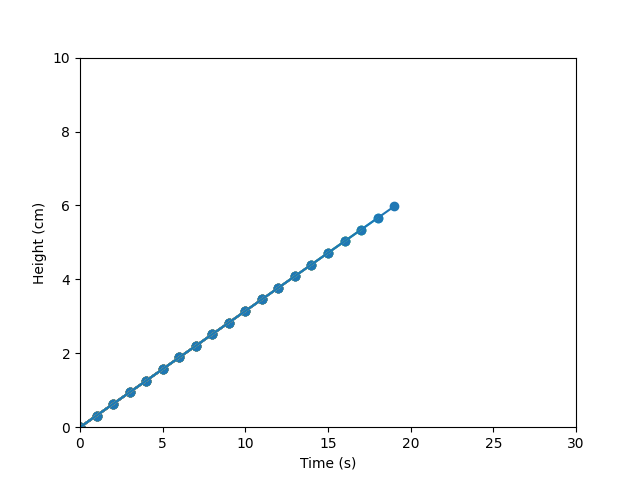
\includegraphics[width=0.75\textwidth]{water-filling-fd.png}
%	\end{figure}
	
	\subsection{Code without Graphical Output}
	A stripped down version of the code with no graph and no external modules except "math".
	
	\textit{water-filling-fd-noGraph.py}
	\lstinputlisting[language=Python, frame=single]{../water-filling-fd-noGraph.py}
	
	
	Which should produce a table of time and height output:
	
	\begin{lstlisting}
0 0
1.0 0.31438013450250935
2.0 0.6287602690050187
3.0 0.943140403507528
4.0 1.2575205380100374
5.0 1.5719006725125468
6.0 1.8862808070150563
7.0 2.2006609415175657
8.0 2.515041076020075
9.0 2.8294212105225847
10.0 3.143801345025094
11.0 3.4581814795276036
12.0 3.772561614030113
13.0 4.086941748532622
14.0 4.4013218830351315
15.0 4.715702017537641
16.0 5.03008215204015
17.0 5.34446228654266
18.0 5.658842421045169
19.0 5.973222555547679
	\end{lstlisting}



\section{Analytical Solutions using Calculus}

	The analytical solution to this problem will help confirm the accuracy of our model.+

	\subsection{Filling}

	As we saw in the section on using calculus (Section \ref{CodeCalc}), we can start with the equation for the volume of a cylinder:
	\begin{equation}
		V = \pi r^2 h
	\end{equation}
	
	And differentiate with respect to time to get:
	\begin{equation}
		\frac{dV}{dt} = \pi r^2 \frac{dh}{dt} 
	\end{equation}

	Assuming a constant inflow rate ($\frac{dV}{dt} = Q$):
	\begin{equation}
		Q = \pi r^2 \frac{dh}{dt} 
	\end{equation}

	And solve for $\frac{dh}{dt}$:
	\begin{equation}
		\frac{dh}{dt} = \frac{Q}{\pi r^2 }
	\end{equation}

	This we can separate:
	\begin{equation}
		dh = \frac{Q}{\pi r^2 } dt
	\end{equation}
	
	and integrate:
	\begin{equation}
		\int{dh} = \int{\frac{Q}{\pi r^2 } dt}
	\end{equation}

	to get:
	\begin{equation}
		h = \frac{Q}{\pi r^2 } t + c
	\end{equation}

	When $t=0$, $c$ can be shown to be the initial height ($c = h_i$) so:
	\begin{equation}
		h = \frac{Q}{\pi r^2 } t + h_i
	\end{equation}

	And since $\frac{Q}{\pi r^2}$ is constant, we can see that this term is the slope in a linear equation of the form.
	\begin{equation}
		y = mx + b
	\end{equation}

	So the linear pattern produced by the filling model is correct (Figure \ref{fillingModel}).



 % Stop your text
 \end{document}
